So far we considered only cases where one game was played once. We would like to study situations where a single game - called the stage game in this context - is
played several times in a row with the assumption that the result of each stage game is observed before the next round is played. Such a game is called
a repeated game. Depending on how often the stage game is repeated one distinguishes between finite and infinite repeated games. Let us introduce this setting
in a more formal manner. Again we restrict ourselves to two games with only two players.

\begin{definition}\label{def:repGame}
    Let $G = (S, \pi)$ be a strategic game, let $\delta \in(0, 1]$ and let $k\in\nats\cup\{\infty\}$. 
    \begin{enumerate}
        \item Let $S^{0} = \{\phi\}$. Then any element $h\in S^{j - 1}$
            is called history at period $j\in\{1, \ldots, k\}$. The set $H = \bigcup_{j = 1}^{k}S^{j - 1}$ is called set of histories.
        \item Let $i = 1, 2$. Then a mapping $\sigma:H\to S_{i}$ is called a strategy of player $i$. The set of strategies of player $i$ is denoted by $\Sigma_{i}$.
        \item Let $\sigma_{1}\in\Sigma_{1}, \sigma_{2}\in\Sigma_{2}$ and let $h\in H$. The pairs $\sigma = (\sigma_{1}, \sigma_{2})$ and $\sigma(h) = (\sigma_{1}(h), \sigma_{2}(h))$
            are called strategy profile and action profile respectively.
        \item Let $\sigma = (\sigma_{1}, \sigma_{2})$ be a strategy profile and let the action profiles $a_{1}, \ldots, a_{k}$ be recursively defined by
            \begin{equation*}
                a_{1}(\sigma) = \sigma(\phi) ~\text{ and }~ a_{j}(\sigma) = \sigma(a_{1}(\sigma), \ldots, a_{j - 1}(\sigma))), 2\leq j\leq k.
            \end{equation*}
            Then the discounted payoff functions $\pi_{i}^{(\delta)}:\Sigma_{1}\times\Sigma_{2}\to\reals$, $i = 1, 2$ are defined by
            \begin{equation*}
                \pi_{i}^{(\delta)}(\sigma_{1}, \sigma_{2}) = \sum_{j = 1}^{k}\delta^{j - 1}\pi_{i}(a_{j}(\sigma))
            \end{equation*}         
        \item The strategic game $G(\delta, k) = (\Sigma, \pi^{(\delta)})$ where $\Sigma = \Sigma_{1}\times\Sigma_{2}$, $\pi^{(\delta)} = (\pi_{1}^{(\delta)}, \pi_{2}^{(\delta)})$ is
            called the $k$-fold repetition of $G$ with discount factor $\delta.$
    \end{enumerate}
\end{definition}

\begin{remark}
    The use of discounted rewards models the assumption that for all the players rewards in the near future are more important than later ones. Additionally
    in the case of $k = \infty$ discounting ensures the welldefinedness of the payoff functions.
\end{remark}

Similar as for non repeated games we define what we understand under a Nash equilibrium. Additinoally we introduce the concept of a subgame perfect equilibrium. Given
$h\in H$, and a repeated game $G(\delta, k) = (\Sigma, \pi^{(\delta)})$ in the sense of Definition \ref{def:repGame}, we denote by $G(\delta, k)_{|h}$ the subgame 
which begins after history $h$. For a strategy profile $\sigma$ the restriction of $\sigma$ to $G(\delta, k)_{|h}$ is denoted by $\sigma_{|h}$.
\begin{definition}
    Let $G(\delta, k) = (\Sigma, \pi^{(\delta)})$ be a repeated game in the sense of Definition \ref{def:repGame}.
    \begin{enumerate}
        \item A strategy profile $\sigma^{*} = (\sigma_{1}^{*}, \sigma_{2}^{*})$ is called a Nash equilibrium if for all
            $\hat{\sigma}_{1}\in\Sigma_{1}, \hat{\sigma}_{2}\in\Sigma_{2}$ holds
            \begin{equation*}
                \pi_{1}^{(\delta)}(\sigma^{*})\geq \pi_{1}^{(\delta)}(\hat{\sigma}_{1}, \sigma_{2}^{*}) ~\text{ and }~
                \pi_{2}^{(\delta)}(\sigma^{*})\geq \pi_{2}^{(\delta)}(\hat{\sigma}_{1}^{*}, \hat{\sigma}_{2})
            \end{equation*}
        \item A strategy profile $\sigma_{*}$ is called a subgame perfect Nash equilibrium if for each $h\in H$ the restricted profile
            $\sigma_{|h}$ is a Nash equilibrium of $G(\delta, k)_{|h}$.
    \end{enumerate}
\end{definition}

\begin{remark}
    A subgame perfect Nash equilibrium is obtained if players choose at every time step the strategy which is maximising their payoff. 
\end{remark}

\begin{example}[The annoying neighbour problem - finitely repeated]
    Let us consider the scenario of two persons, Florian and Laurent, living next to each other. Florian likes to stand up early and listen to metal music, 
    whereas Laurent likes to go to bed rather late and listen to classical music. Unfortunately, the walls between the apartments are very thin, so both 
    Florian and Laurent can hear each other's music. Thus if Laurent listens to music Florian can't sleep and on the other way round Laurent wakes up early
    if Florian is listening to his favorite music in the morning. Both of them have the option to listen to their favorite music quite ($q$) or loud ($l$). 
    If Florian listens to loud music, and Laurent, on the other hand, only listens to music quietly, Laurent is in a bad mood because he has tried to be
    considerate and Florian has not - the same holds the other way round. We model the situation by means of a strategic game descrived by means of the 
    following table
    \begin{center}
        \begin{tabular}{c | r | c | c |}
            \multicolumn{2}{c}{} & \multicolumn{2}{c}{Laurent}\\
            \cline{2-4}
            & & $q$ & $l$ \\
            \cline{2-4}
            \multirow{2}{*}{Florian} & $q$ & (2, 2) & (-3, 3) \\
            \cline{2-4}
            & $l$ & (3, -3) & (-2, -2)) \\
            \cline{2-4}
        \end{tabular}            
    \end{center}
    Let us consider the situation where the game is played twice, i.e. at time $t = 1$ the neighbours decide how they want to listen to music and, knowing 
    the result of this first round they may decide again at time $t = 2$. We try to find a subgame perfect Nash equilibrium by means of backward induction: We 
    first analyse the situation at the final stage, i.e. at time $t = 2$. Given for example the stage strategy pair $(q, q)$ at time $t = 1$, and assuming that
    Florian opts for $q$, where Laurent chooses $l$ we get the the payoffs $2 -3 \delta$ and $2 + 3\delta$ for Florian and Laurent respectively. Let us list
    all the possible strategy combinations and the corresponding payoffs using the following table
    \begin{center}
        \begin{tabular}{| c | c | c |}
            \cline{1 - 3}
            $t = 1$ & $t = 2$ & cumulative payoff \\
            \cline{1 - 3}
            % (q, q)
            $(q, q)$ & $(q, q)$ & $(2 + 2\delta, 2 + 2\delta)$ \\
            $(q, q)$ & $(q, l)$ & $(2 - 3\delta, 2 + 3\delta)$ \\
            $(q, q)$ & $(l, q)$ & $(2 + 3\delta, 2 - 3\delta)$ \\
            $(q, q)$ & $(l, l)$ & $(2 - 2\delta, 2 - 2\delta)$ \\
            \cline{1 - 3}
            % (q, l)
            $(q, l)$ & $(q, q)$ & $(-3 + 2\delta, 3 + 2\delta)$ \\
            $(q, l)$ & $(q, l)$ & $(-3 - 3\delta, 3 + 3\delta)$ \\
            $(q, l)$ & $(l, q)$ & $(-3 + 3\delta, 3 - 3\delta)$ \\
            $(q, l)$ & $(l, l)$ & $(-3 - 2\delta, 3 - 2\delta)$ \\
            \cline{1 - 3}
            % (l, q)
            $(l, q)$ & $(q, q)$ & $(3 + 2\delta, -3 + 2\delta)$ \\
            $(l, q)$ & $(q, l)$ & $(3 - 3\delta, -3 + 3\delta)$ \\
            $(l, q)$ & $(l, q)$ & $(3 + 3\delta, -3 - 3\delta)$ \\
            $(l, q)$ & $(l, l)$ & $(3 - 2\delta, -3 - 2\delta)$ \\
            \cline{1 - 3}
            % (l, q)
            $(l, l)$ & $(q, q)$ & $(-2 + 2\delta, 2 + 2\delta)$ \\
            $(l, l)$ & $(q, l)$ & $(-2 - 3\delta, 2 + 3\delta)$ \\
            $(l, l)$ & $(l, q)$ & $(-2 + 3\delta, 2 - 3\delta)$ \\
            $(l, l)$ & $(l, l)$ & $(-2 - 2\delta, 2 - 2\delta)$ \\
            \cline{1 - 3}
        \end{tabular}            
    \end{center}
    The first column gives the strategy pairs at $t = 1$ and the second column shows the strategy pairs $t = 2$. The third column contains the corresponding
    cumulative payoffs. We infer that independent of the player's strategies in the first stage, neither Laurent nor Florian benefit if unilaterally deviating
    from the strategy $q$. Thus, we proved that the strategies of both players mapping each history to $l$ build a subgame perfect Nash equilibrium.
\end{example}

Using the same reasoning as in the above example one can easily prove the following theorem.
\begin{theorem}
    Let $G = (S, \pi)$ be a strategic game with a single pure Nash equilibrium $s^{*}$. Let $k\in\nats$ and let $\delta > 0$. The strategy profile given by
    $\sigma = (\sigma_{1}^{*}, \sigma_{2}^{*})$, where $\sigma_{i}^{*}(h) = s^{*}$ for every $i = 1, 2$, $h\in H$ is the unique Nash equilibrium of the 
    $k$-fold repeated game $G(\delta, k)$.
\end{theorem}

\begin{remark}
    Theorems giving conditions on the existence of Nash equilibria of repeated games are known as Folk Theorems. 
\end{remark}

\begin{example}[The annoying neighbour problem - infinitely repeated]
    Let us assume that the game gets repeated infinitely often. We do not want to discuss the problem theoretically. Instead we try to find numerically strategies which 
    perform best. We use an approach presented in \cite{mathieu2017new} which is based on a evolutionary competition of a given set of $n$ strategies. In the first generation 
    a set of players of cardinality larger than $n$ is generated in such a way that the strategies are distributed equally among the players and each player is assigned exactly
    one strategy. In a tournament, all players compete against each other for a fixed number of repetitions of the stage game. Based on the resulting cumulative payoffs,
    the players (or the performance of the associated strategies) are evaluted. This ranking is used to procure a second generation from the first generation. This second generation
    consists of the same total number of players, with the distribution of the strategies among the players being determined from the results of the tournament of the previous generation.
    The better the strategy, the greater the proportion of players with that same strategy in the new generation. This process is repeated for a fixed number of generations.
    \begin{figure}[h!]
        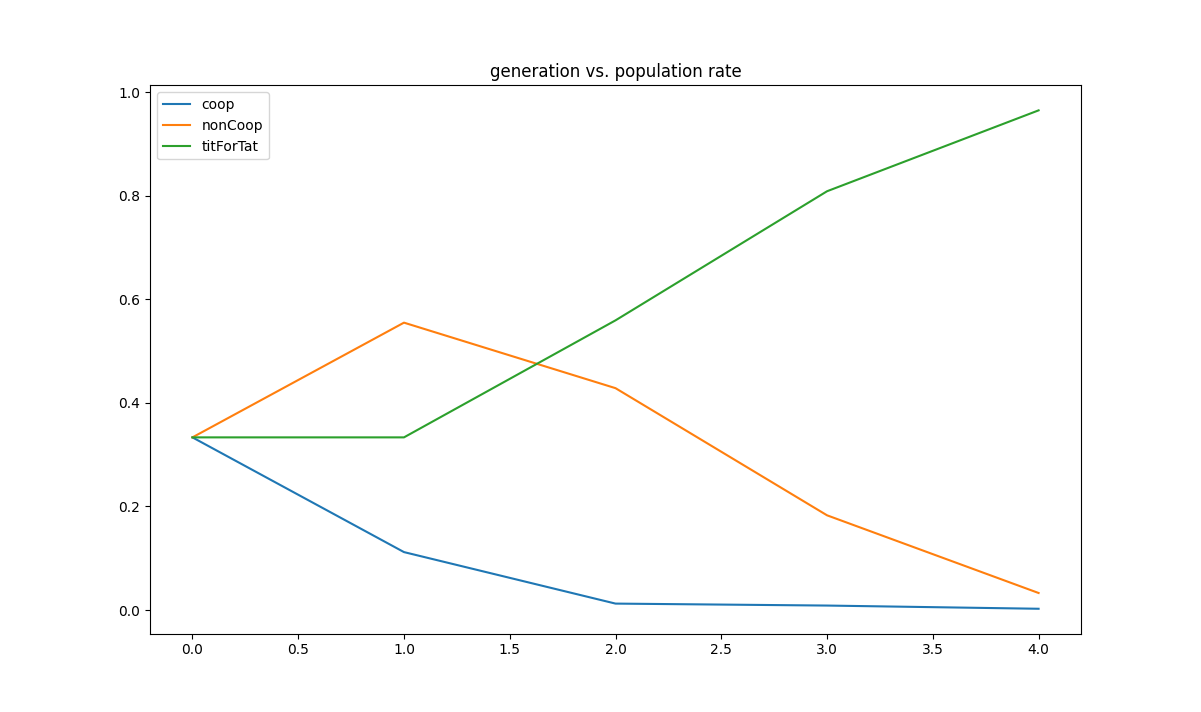
\includegraphics[width = 0.75\textwidth]{images/performance_strategies_repeated}
        \centering
        \caption{The figures shows the performance of the three strategies 'cooperation', 'no cooperation', and 'tit for tat'.}
    \end{figure}
\end{example}
